\documentclass{article}

\usepackage{graphicx}
\usepackage{subcaption}
\usepackage{tikz}
\usepackage[utf8]{inputenc}
\usepackage[T1]{fontenc}
\usepackage{lmodern}
\usepackage{amsmath}
\usepackage{amsthm}
\usepackage{amsfonts}
\usepackage{amssymb}
\usepackage{enumitem}
\usepackage{commath}
\usepackage{mathtools}
\usepackage{adjustbox}
\usepackage{setspace}
\usepackage{bigints}
\usepackage{hyperref}
\usepackage{ulem}
\usepackage{esdiff}
\usepackage{pgfplots}
\usepackage{caption}
\usepackage{tikz-cd}
\usetikzlibrary{shapes.symbols}
\usetikzlibrary{calc,patterns,angles,quotes}

\newtheorem{definicija}{Definicija}
\newtheorem{trditev}{Trditev}
\newtheorem{lema}{Lema}
\newtheorem{posledica}{Posledica}
\newtheorem{opomba}{Opomba}
\newtheorem{primer}{Primer}
\newtheorem{izrek}{Izrek}


\newcommand{\C}{\mathbb{C}}
\newcommand{\D}{\mathbb{D}}
\newcommand{\Z}{\mathbb{Z}}
\newcommand{\N}{\mathbb{N}}
\newcommand{\M}{\mathcal{M}}
\newcommand{\F}{\mathcal{F}}
\newcommand{\R}{\mathbb{R}}
\newcommand{\Ho}{\mathcal{O}}
\newcommand{\dd}{\mathrm{d}}


\title{Zvezna dinamični sistemi - lokalni del}
\author{Uroš Kosmač}

\begin{document}
\maketitle

Obravnavali bomo nelinearne avtonomne sisteme navadnih diferencilnih enačb (NDE)
t.j. 
\begin{equation}
\dot{X} = F(X),
\end{equation}
kjer so $U \subset \R^n$ odprta, $F:U \rightarrow R^n$ in $X: I \subset \R \rightarrow \R^n$
vektorska funckija. 

\begin{primer}
Matematično nihalo
\begin{center}
    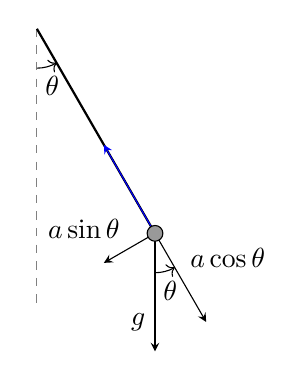
\begin{tikzpicture}
        % save length of g-vector and theta to macros
        \pgfmathsetmacro{\Gvec}{1.5}
        \pgfmathsetmacro{\myAngle}{30}
        % calculate lengths of vector components
        \pgfmathsetmacro{\Gcos}{\Gvec*cos(\myAngle)}
        \pgfmathsetmacro{\Gsin}{\Gvec*sin(\myAngle)}
    
        \coordinate (centro) at (0,0);
        \draw[dashed,gray,-] (centro) -- ++ (0,-3.5) node (mary) [black,below]{$ $};
        \draw[thick] (centro) -- ++(270+\myAngle:3) coordinate (bob);
        \pic [draw, ->, "$\theta$", angle eccentricity=1.5] {angle = mary--centro--bob};
        \draw [blue,-stealth] (bob) -- ($(bob)!\Gcos cm!(centro)$);
        \draw [-stealth] (bob) -- ($(bob)!-\Gcos cm!(centro)$)
          coordinate (gcos)
          node[midway,above right] {$a\cos\theta$};
        \draw [-stealth] (bob) -- ($(bob)!\Gsin cm!90:(centro)$)
          coordinate (gsin)
          node[midway,above left] {$a\sin\theta$};
        \draw [-stealth] (bob) -- ++(0,-\Gvec)
          coordinate (g)
          node[near end,left] {$g$};
        \pic [draw, ->, "$\theta$", angle eccentricity=1.5] {angle = g--bob--gcos};
        \filldraw [fill=black!40,draw=black] (bob) circle[radius=0.1];
    \end{tikzpicture}
\end{center}
$2$. Newtonov zakon
\begin{align*}
ma &= -F \\
m\ddot{\varphi} &= -mg \\
\ddot{\varphi} + &g\sin{\varphi} = 0
\end{align*}
Začetni pogoj:
\begin{align*}
\varphi(0) &= \varphi_0\,\, \text{ začetni odmik }\\
\dot{\varphi}(0) &= v_0 \,\, \text{ začetna hitrost }
\end{align*}
Začetni problem je NDE oz. sistem NDE skupaj z začetnim pogojem.
To želimo obravnavati kot sistem prvega reda, zato bomo enačbo
drugega reda prevedli nanj. Zaradi enostavnosti nastavimo $g = 1$.
\begin{align*}
x = \varphi \\
y = \dot{\varphi} ... 
\end{align*}
Začetni pogoj je 
$$
\binom{x}{y}(0) = \binom{\varphi}{\dot{\varphi}} = \binom{\varphi_0}{v_0}.
$$
Za začetek si oglejmo linearizacijo tega sistema t.j. uporabimo oceno
$\sin{x} \approx x$ za majhen $x$:
\begin{align*}
\binom{\dot{x}}{\dot{y}} = \binom{y}{-x} = A\binom{x}{y}.
\end{align*}
Ni težko preveriti, da je splošna rešitev enaka:
\begin{align*}
\binom{\dot{x}}{\dot{y}} = \binom{c\cos{t} + D\sin{t}}{-C\sin{t} + D\cos{t}}
\end{align*}
Pri danem začetnem pogoju dobimo $x(0) = C = x_0$ in $y(0) = D = y_0$. 
Opazimo tudi, da za vse začetne pogoje $x_0, y_0 \in \R$ ter $t\in \R$
velja:
$$
x^2 + y^2 = ... = x_0^2 + y_0^2.
$$
To pomeni, da vsaka rešitev sistema leži znotraj glavne krožnice 
s polmerom $\sqrt{x_0^2 + y_0^2}$. To ne pomeni nujno, da opišemo celotno 
krožnico, vendar pa je v našem primeru to jasno iz parametrizacije.\\
Tokovnice\\
\begin{itemize}
    \item Tovrstnim upodobitvam rešitev za razžične začetne pogoje 
    pravimo \textbf{fazni portret}.
    \item Krivuljam v portretu pravimo \textbf{orbite}, \textbf{tokovnice} ali \textbf{trajektorije}.
    \item Zvezi $G(X) \equiv C\in\R$, ki velja "za vse smiselne čase"
    in vse rešitve, pravimo \textbf{prvi integral sistema}.
\end{itemize}
Lineariziran sistem ima dva tipa rešitev:
\begin{itemize}
    \item \textbf{Ravnovesno oz. stacionarno točko} v izhodišču t.j.
    točko $x_0$, v kateri je $F(X_0) = 0$. Tam sistem miruje.
    \item \textbf{Periodične rešitve} pri katerih obstaja $T>0$, da je 
    $X(t + T) = x(t)$ za vse smiselne čase in je $T$ najmanjši s to lastnostjo. 
    V našem primeru $T = 2\pi$.
\end{itemize}
Poglejmo si sedaj nelinearn sistem.
\begin{align*}
\binom{\dot{x}}{\dot{y}} = \binom{y}{-\sin{x}} = F(x, y).
\end{align*}
Sistema neznamo rešiti eksplicitno, znamo pa poiskati prvi integral.
Če nismo ravno v "slabi točki", lahko vsaj na okolici izrazimo 
$y = y(x)$. Za odvod pa velja 
$$
y' = \frac{\dif y}{\dif x} = \frac{\frac{\dif y}{\dif t}}{\frac{\dif x}{\dif t}} = \frac{\dot{y}}{\dot{x}}.
$$
V našem primeru: 
$$
\frac{\dif y}{\dif x} = \frac{\dot{y}}{\dot{x}} = - \frac{\sin{x}}{y}.
$$
Dobili smo NDE z ločjivimi spremenljivkami
\begin{align*}
\int y \dif y &= - \int \sin{x} \dif x\\
\frac{y^2}{2} &= \cos{x} + \tilde{C} \\
y &= \pm \sqrt{2\cos{x} + C}
\end{align*}
Ta zveza podaja obliko unije tokovnic, ne pa nujno tudi tokovnic samih.\\
vfasv<f\\
Smer toka določa enačba $\dot{x} = y$. Ugotovimo, da lahko analizaramo obnašanje sistema 
čeprav ne poznamo eksplicitno rešitev sistema. To bo cilj tega in naslednjega poglavja.
Poleg ravnovesnih in periodičnih rešitev smo v tem primeru dobili tudi neperiodično 
za $C > 2$. Dodatno opazimo, da so ravnovesne točke v $(k\pi, 0)$
$k\in \Z$, vendar pa so dbeh tipov:
\begin{enumerate}
    \item[->] za $k$ sod stabilne
    \item[->] za $k$ lih nestabilne
\end{enumerate}
\end{primer}

\begin{definicija}
Ravnovesna točka $X_0$ je \textbf{stabilna}, če za vsako njeno okolico 
$U \subset \R^n$ obstaja manjša okolica $V \subset U$, da za rešitev 
z lastnostjo $X(0) \in V$ velja $X(t) \in U$ za vse $t > 0$. Če 
dodatno velja tudi
$$
\lim_{t\rightarrow \infty} X(t) = X_0, 
$$
je točka tudi \textbf{asimptotsko stabilna}.
\end{definicija}
V našem primeru imamo le stabilnost. \\
domenice\\
Opazimo, da je lineariziran portret "zelo podobne" originarini 
okokici $(0, k\pi)$ za sode $k\in \Z$. To bo stabilno tudi za zvezne 
verzije Hartman-Grobmanovega izreka, ki je cilj tega poglavja.

\section{Eksistenčni izrek in tok sistema}

V tem razdelku bomo razširili že poznan eksistenčnio izrek za NDE.
Spomnimo se: iskali smo rešitev začetnega problema
\begin{align*}
\dot{x} &= f(t, x) \\
x(t_0) &= x_0
\end{align*}
vsaj na okolici začetne točke t.j. za $t\in (t_0 - a, t_0 + a)$.
Izkazalo se je , da je za obstoj rešitve dovolj zveznost funckije $f$ za
enoličnost pa so potrebni dodatni pogoji. 
\begin{primer}
\begin{align*}
\dot{x} &= 3x^\frac{2}{3} \\
x(0) &= 0. 
\end{align*}
Rešitvi sta $x(t) = 0$ in $x(t) = t^3$.
\end{primer}
Zaradi zadnjega primera se v izreku prevzame Lipshitzova lasntnost t.j.
$$
|f(t, x_1) - f(t, x_2)| < L |x_1 - x_2|\,\, \text{ za } L>0.
$$
Ta lastnost mora držati na okolici točke $(t_0, x_0)$.
Zadosten pogoj je bil $C^1$-odvedljivost po spremenljivki $x$.
Reševali bomo začetni problem: 
$$
\dot{X} = F(X),\,\, X(0) = x_0,
$$
kjer smo se omejili na avtonomne sisteme. Rešitev bomo iskali v prostoru:
$$
C([-a, a], \R^n).
$$
Privzeli bomo, da je $U \subseteq \R^n$ vedno odprta in $F \in C^1(U)$
t.j. $F = (F_1, \dots, F_n): U \rightarrow \R^n$ vsaka koordinatna 
funckija $F_j$ je zvezno odvedljiva po vseh $x_k$, $1 \leq k \leq n$.

\begin{lema}
Naj bo $U \subset \R^n$ odprta, $x_0 \in U$ in $F\in C^1(U)$.
Potem obstajata $R > 0$ in $L > 0$, da $\forall x_1, x_2 \in \mathbb{B}(X_0, \R)$
velja 
$$
|F(X_1) - F(X_2)| < L|X_1 - X_2|.
$$
\end{lema}

\begin{proof}[Dokaz:]
    Naj bo $R > 0$ tak, da je $\overline{\mathbb{B}(x_0, R)} \subset U$
    in naj bo 
    $$
    L \coloneqq \max_{x\in \overline{\mathbb{B}(X_0, R)}} ||D_F(X)||
    $$
    največja operatorska norma Jacobijeve matrike. Zaradi konveksnosti $\mathbb{B}$, je za  $X_1, X_2 \in \mathbb{B}(x_0, R)$, je 
    $X_1 \cdot s + X_2(1 - s) \in \mathbb{B}(X_0, R)$ in $s\in [0, 1]$.
    Definiramo preslikavo ene spremenljivke:
    \begin{align*}
    g(s) &= F(X_2 + sV), \,\, V = X_1 - X_2, \,\, s\in [0, 1]
    g'(s) &= D_F(X_2 + sV) \cdot V
    \end{align*}
    Od tod sledi:
    $$
    |g'(s)| \leq L \cdot |V| = L\cdot |X_1 - X_2|.
    $$
    Običajen Langrangeov izrek za vektorske funckije pove:
    $$
    |F(X_1) - F(X_2)| = |g(0) - g(1)| = |g'(s)| \leq L |X_1 - X_2|.
    $$
\end{proof}

\begin{opomba}
Iz dokaza je razvidno, da bi lahko namesto $\mathbb{B}(X_0, R)$
uporabili poljubno množico, ki je kompaktno vsebovana v $U$, 
potrebujemo zgolj konveksnost. Vendar se izkaže, da je tudi ta predpostavka 
odveč, saj lahko najdemo konveksno končno pokritje.
\end{opomba}

Sklep: za vsako kompaktno $K \subset U$ obstaja $L > 0$, da je 
$$
|F(x_1) - F(X_2)| < L |X_1 - X_2|
$$
za $X_1, X_2 \in K$ t.j. $F\in C^1(U)$ je Lipshitzova na vsakem 
kompaktu v $U$. Izkaže se, da ke ta pogoj dovolj za konvergenco 
Picardove iteracije 
\begin{align*}
\dot{X} &= F(X) \\
\dot{X}(0) = X_0 \iff &\underbrace{X(t) = X_0 + \int_0^t F(X(\tau)) \dif \tau}_{\text{integralska oblika začetnega pogoja}} \\
\end{align*}

TBA\\[2mm]

Picardova iteracija:
$$
x_n = \Phi(x_{n-1}), \,\, X_0(x) = X_0.
$$
Iteracija bo konvergirala, če bo obstajala fiksna točka $\Phi(x) = x$,
saj to reši začetni problem.

\begin{izrek}
Naj bodo $F\in C^1(U)$, $X_0 \in U$, $\dot{X} = F(X)$ in $X(0) = X_0$.
Potem ima začetni problem enolično zvezno rešitev, ki je definirana 
za $t\in [-a, a]$ za nek $a > 0$.
\end{izrek}

\begin{proof}[Dokaz:]
Dobolj je dokazatim, da ima $\Phi$ fiksno točko oz. da je skrčitev 
na ustrezno izbranem polnem prostoru. 
\begin{itemize}
    \item Naj bo $F$ Lipshitzova na $\overline{B(0, R)} \subset U$
    za konstanto $L>0$ in naj bo $M \coloneqq \max_{x\in\overline{B(0, R)}} |F(X)|$.
    \item Prostor $C^1([-a, a], \R^n)$ opremimo z metriko $d_\infty$, 
    ter se omejimo na $\mathcal{K} \subset C^1([-a, a], \R^n)$, v 
    kateri so funkcije z lastnostjo: $|X(t) - X_0| \leq R$
    za vse $t\in [-a, a]$.
    \item Prostor $(\mathcal{K}, d_\infty)$ je poln za vsak $a>0$. 
    \item Trdimo, da za dovolj majhen $a>0$, velja $\Phi(\mathcal{K}) \subseteq \mathcal{K}$.
    \begin{align*}
    |\Phi(X)(t) - X_0| &= \| \int_0^t F(X(\tau)) \dif \tau \| \leq \\
                       &\leq 2a\cdot M\leq R \Longrightarrow a \leq \frac{R}{M}.
    \end{align*}
    \item Trdimo, da je za dovolj majhen $a>0$ $\Phi$ skrčitev:
    \begin{align*}
    d_\infty(\Phi(X), \Phi(\tilde{X})) = \max_{t\in [-a, a]} \|\|
    \end{align*}
\end{itemize}


\end{proof}



\end{document}